\documentclass[../../../analisi-dei-requisiti.tex]{subfiles}

\begin{document}

\begin{figure}[H]
  \centering
  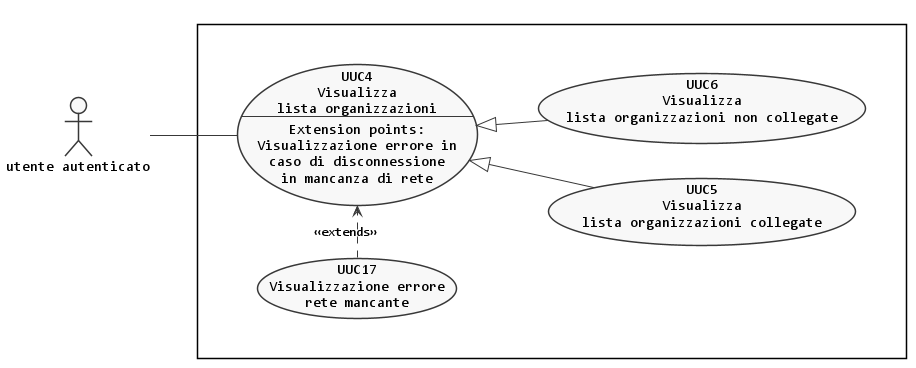
\includegraphics[width=150mm]{gestione-lista-organizzazioni.png}
  \caption{UUC4: Gestione lista organizzazioni}%
  \label{fig:uuc4}
\end{figure}

\begin{description}
  \item[Caso d’uso:] UUC4;
  \item[Titolo:] Gestione lista organizzazioni;
  \item[Attori primari:] utente autenticato;
  \item[Precondizione:] l'utente visualizza la pagina relativa al recupero delle organizzazioni;
  \item[Postcondizione:] l'utente seleziona una o più organizzazioni;
  \item[Scenario principale:]
        \begin{enumerate}
          \item l'utente ha la possibilità di recuperare una lista di organizzazioni alla quale si può collegare.
        \end{enumerate}
  \item[Estensioni:]
        \begin{enumerate}
          \item in caso di rete mancante, non possono essere eseguite queste operazioni e quindi verrà notificato un errore~\ref{subs:UUC12};
          \item in caso l'organizzazione sia privata, è richiesta l'autenticazione da parte dell'utente~\ref{subs:UUC4.3}.
        \end{enumerate}
\end{description}


\subsubsection{UUC4.1: Aggiornamento lista organizzazioni}%
\label{subs:UUC4.1}
\begin{description}
  \item[Caso d’uso:] UUC4.1;
  \item[Titolo:] Aggiornamento lista organizzazioni;
  \item[Attori primari:] utente autenticato;
  \item[Precondizione:] l'utente visualizza la lista delle organizzazioni;
  \item[Postcondizione:] l'utente ha aggiornato la lista delle organizzazioni;
  \item[Scenario principale:]
        \begin{enumerate}
          \item l'utente ha la possibilità di aggiornare la lista delle organizzazioni, e viene avvisato mediante \glossario{notifica} dell'applicazione mobile.
        \end{enumerate}
  \item[Estensioni:]
        \begin{enumerate}
          \item in caso di rete mancante, non può essere eseguito l'aggiornamento della lista di organizzazioni e quindi verrà notificato un errore~\ref{subs:UUC12}.
        \end{enumerate}
\end{description}


\subsubsection{UUC4.2: Seleziona organizzazioni}%
\label{subs:UUC4.2}
\begin{description}
  \item[Caso d’uso:] UUC4.2;
  \item[Titolo:] Seleziona organizzazioni;
  \item[Attori primari:] utente autenticato;
  \item[Precondizione:] l'utente visualizza la lista delle organizzazioni;
  \item[Postcondizione:] l'utente ha selezionato una o più organizzazioni;
  \item[Scenario principale:]
        \begin{enumerate}
          \item l'utente ha la possibilità di selezionare una o più organizzazioni.
        \end{enumerate}
  \item[Estensioni:]
        \begin{enumerate}
          \item in caso di rete mancante, non possono essere selezionate organizzazioni e quindi verrà notificato un errore~\ref{subs:UUC12};
          \item in caso l'organizzazione alla quale l'utente vuole autenticarsi sia privata, è richiesta l'autenticazione~\ref{subs:UUC4.3}.
        \end{enumerate}
\end{description}

\begin{figure}[H]
  \centering
  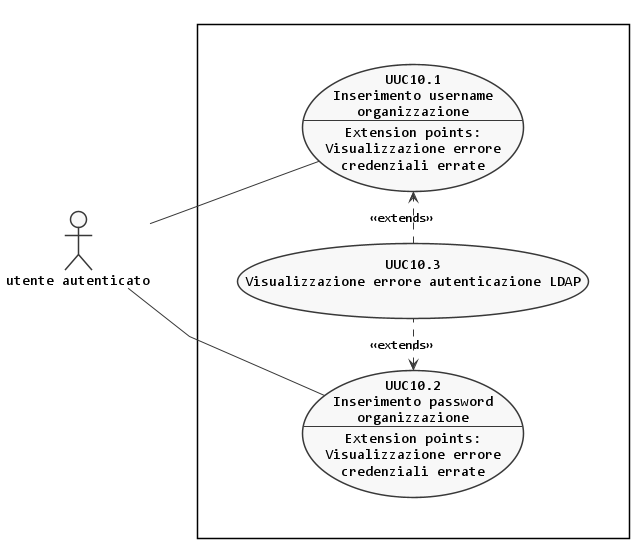
\includegraphics[width=150mm]{autenticazione-ldap-organizzazione.png}
  \caption{UUC4.3: Autenticazione LDAP organizzazione}%
  \label{fig:uuc4.3}
\end{figure}

\subsubsection{UUC4.3: Autenticazione LDAP organizzazione}%
\label{subs:UUC4.3}
\begin{description}
  \item[Caso d’uso:] UUC4.3;
  \item[Titolo:] Autenticazione organizzazione;
  \item[Attori primari:] utente autenticato;
  \item[Attori secondari:] server LDAP\@;
  \item[Precondizione:] l'utente ha selezionato un'organizzazione privata;
  \item[Postcondizione:] l'utente è autenticato all'organizzazione privata e diventa un utente collegato noto;
  \item[Scenario principale:]
        \begin{enumerate}
          \item l'utente ha selezionato un'organizzazione privata, in quanto la tracciatura prevista è nota.
          \item l'utente deve autenticarsi all'organizzazione privata tramite il server LDAP, inserendo le credenziali rilasciate dall'organizzazione e univoche per tutti gli utenti interessati ad essere monitorati.
        \end{enumerate}
  \item[Estensioni:]
        \begin{enumerate}
          \item se le credenziali inserite dall'utente non corrispondono a quelle dell'organizzazione, allora visualizzerà un errore~\ref{subs:UUC4.3.3}.
        \end{enumerate}
\end{description}

\subsubsection{UUC4.3.1: Inserimento username organizzazione}%
\label{subs:UUC4.3.1}
\begin{description}
  \item[Caso d’uso:] UUC4.3.1;
  \item[Titolo:] Inserimento username organizzazione;
  \item[Attori primari:] utente autenticato;
  \item[Attori secondari:] server LDAP\@;
  \item[Precondizione:] l'utente non ha ancora inserito lo username dell'organizzazione;
  \item[Postcondizione:] l'utente ha inserito lo username dell'organizzazione;
  \item[Scenario principale:]
        \begin{enumerate}
          \item l'utente inserisce lo username relativo all'organizzazione privata alla quale vuole collegarsi;
        \end{enumerate}
  \item[Estensioni:]
        \begin{enumerate}
          \item se lo username inserito dall'utente non corrisponde a quello dell'organizzazione, allora visualizzerà un errore~\ref{subs:UUC4.3.3}.
        \end{enumerate}
\end{description}

\subsubsection{UUC4.3.2: Inserimento password organizzazione}%
\label{subs:UUC4.3.2}
\begin{description}
  \item[Caso d’uso:] UUC4.3.2;
  \item[Titolo:] Inserimento password organizzazione;
  \item[Attori primari:] utente autenticato;
  \item[Attori secondari:] server LDAP\@;
  \item[Precondizione:] l'utente non ha ancora inserito la password dell'organizzazione;
  \item[Postcondizione:] l'utente ha inserito la password dell'organizzazione;
  \item[Scenario principale:]
        \begin{enumerate}
          \item l'utente inserisce la password relativa all'organizzazione privata alla quale vuole collegarsi;
        \end{enumerate}
  \item[Estensioni:]
        \begin{enumerate}
          \item se la password inserita dall'utente non corrisponde a quella dell'organizzazione, allora visualizzerà un errore~\ref{subs:UUC4.3.3}.
        \end{enumerate}
\end{description}

\subsubsection{UUC4.3.3: Visualizzazione errore autenticazione LDAP}%
\label{subs:UUC4.3.3}
\begin{description}
  \item[Caso d’uso:] UUC4.3.3;
  \item[Titolo:] Visualizzazione errore autenticazione LDAP\@;
  \item[Attori primari:] utente autenticato;
  \item[Attori secondari:] server LDAP\@;
  \item[Precondizione:] i dati forniti dall'utente non corrispondono a credenziali valide;
  \item[Postcondizione:] l'applicazione mobile comunica all'utente il fallimento dell'autenticazione;
  \item[Scenario principale:]
        \begin{enumerate}
          \item l'utente cerca di effettuare l'autenticazione LDAP all'organizzazione privata con credenziali errate.
        \end{enumerate}
\end{description}

\end{document}